\problemset{Introduction to modeling and verification of digital systems}
\problemset{Exercises №1 (revisions)}

\vspace{0.5cm}



\begin{problem}
	Synthesis of a combinational circuit (decoder).
\end{problem}

\begin{proof}
	\hfill
	\begin{center}
		\begin{tabular}{ |C|C|C|C|C|C| } 
			\hline
			A & B & D_0 & D_2 & D_3 & D_4 \\
			\hline
			0 & 0 & 1 & 0 & 0 & 0 \\
			0 & 1 & 0 & 1 & 0 & 0 \\
			1 & 0 & 0 & 0 & 1 & 0 \\
			1 & 1 & 0 & 0 & 0 & 1 \\
			\hline
		\end{tabular}
		\hspace{0.5cm}
		\begin{tabular}{ L } 
			D_0 = \bnot{a} \, \bnot{b} = \bnot{a + b} \\
			D_1 = \bnot{a}b \\
			D_2 = a\bnot{b} \\
			D_3 = ab \\
		\end{tabular}
	\end{center}
\end{proof}



\begin{problem}
	Synthesis of a combinational circuit (priority encoder).
\end{problem}

\begin{proof}
	Let us use a "naive" approach and look at groups of minterms instead of the whole table:
	\begin{center}
		\begin{tabular}{ |C|C|C|C|C|C|C| } 
			\hline
			A_0 & A_1 & A_2 & A_3 & S_0 & S_1 & V \\
			\hline
			0 & 0 & 0 & 0 & 0 & 0 & 0 \\
			0 & 0 & 0 & 1 & 0 & 0 & 1 \\
			0 & 0 & 1 & 0 & 0 & 1 & 1 \\
			0 & 0 & 1 & 1 & 0 & 1 & 1 \\
			0 & 1 & 0 & 0 & 1 & 0 & 1 \\
			0 & 1 & 0 & 1 & 1 & 0 & 1 \\
			0 & 1 & 1 & 0 & 1 & 0 & 1 \\
			0 & 1 & 1 & 1 & 1 & 0 & 1 \\
			1 & 0 & 0 & 0 & 1 & 1 & 1 \\
			1 & 0 & 0 & 1 & 1 & 1 & 1 \\
			1 & 0 & 1 & 0 & 1 & 1 & 1 \\
			1 & 0 & 1 & 1 & 1 & 1 & 1 \\
			1 & 1 & 0 & 0 & 1 & 1 & 1 \\
			1 & 1 & 0 & 1 & 1 & 1 & 1 \\
			1 & 1 & 1 & 0 & 1 & 1 & 1 \\
			1 & 1 & 1 & 1 & 1 & 1 & 1 \\
			\hline
		\end{tabular}
		\hspace{0.5cm}
		\begin{tabular}{ l } 
			$V = \bnot{A_0} \, \bnot{A_1} \, \bnot{A_2} \, \bnot{A_3}$ \\
			\hspace{0.5cm} As we can see: \\
			\hspace{0.5cm} \tabitem $S_0 = A_0$ \\
			\hspace{0.5cm} \tabitem $S_0 = \bnot{A_0} \, A_1$ \\
			$S_0 = A_0 + A_1$ \\
			\hspace{0.5cm} As we can see: \\
			\hspace{0.5cm} \tabitem $S_1 = A_0$ \\
			\hspace{0.5cm} \tabitem $S_1 = \bnot{A_0} \, \bnot{A_1} \, A_2$ \\
			$S_1 = A_0 + \bnot{A_1} \, A_2$ \\
		\end{tabular}
	\end{center}

\vspace{0.3cm}
Priority encoders are often used for:
\begin{itemize}
	\item Encoding keyboard input as ASCII characters (only one key can be triggered at a time in that case).
	\item Encoding data received from a compass to binary (each side has it's own value).
	\item Interruption (IRQ) handling, each interruption has it's own number, the most important of them come first.
\end{itemize}
\end{proof}



\begin{problem}
	Comparison of two combinational circuits.
\end{problem}

\begin{proof}
	Let us enumerate circuit elements:

	\begin{figure}
		\centering
		\textbf{Circuit 1}\par\medskip
		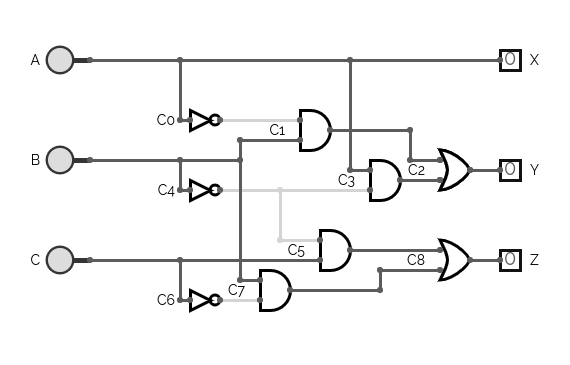
\includegraphics[width=0.5\textwidth]{circuit1}
	\end{figure}
	\begin{center}
		\begin{tabular}{ |C|C|C|C|C|C|C|C|C|C|C|C|C|C|C| } 
			\hline
			A & B & C & C_0 & C_1 & C_2 & C_3 & C_4 & C_5 & C_6 & C_7 & C_8 & X & Y & Z \\
			\hline
			0 & 0 & 0 & 1 & 0 & 0 & 0 & 1 & 0 & 1 & 0 & 0 & 0 & 0 & 0 \\
			0 & 0 & 1 & 1 & 0 & 0 & 0 & 1 & 1 & 0 & 0 & 1 & 0 & 0 & 1 \\
			0 & 1 & 0 & 1 & 1 & 1 & 0 & 0 & 0 & 1 & 1 & 1 & 0 & 1 & 1 \\
			0 & 1 & 1 & 1 & 1 & 1 & 0 & 0 & 0 & 0 & 0 & 0 & 0 & 1 & 0 \\
			1 & 0 & 0 & 0 & 0 & 1 & 1 & 1 & 0 & 1 & 0 & 1 & 1 & 1 & 0 \\
			1 & 0 & 1 & 0 & 0 & 1 & 1 & 1 & 1 & 0 & 0 & 1 & 1 & 1 & 1 \\
			1 & 1 & 0 & 0 & 0 & 0 & 0 & 0 & 0 & 1 & 1 & 1 & 1 & 0 & 1 \\
			1 & 1 & 1 & 0 & 0 & 0 & 0 & 0 & 0 & 0 & 0 & 0 & 1 & 0 & 0 \\
			\hline
		\end{tabular}
		\hspace{0.5cm}
		\begin{tabular}{ l } 
			\hspace{0.5cm} It is obvious that: \\
			$X = A$ \\
			\hspace{0.5cm} Let us calculate: \\
			$Y = \bnot{A} \, B \, \bnot{C} + \bnot{A} \, B \, C + A \, \bnot{B} \, \bnot{C} + A \, \bnot{B} \, C =$ \\
			\hspace{0.25cm} $ = \bnot{A} \, B \, (\bnot{C} + C) + A \, \bnot{B} \, (\bnot{C} + C) =$ \\
			\hspace{0.25cm} $ = \bnot{A} \, B + A \, \bnot{B} = A \oplus B$ \\
			$Z = \bnot{A} \, \bnot{B} \, C + \bnot{A} \, B \, \bnot{C} + A \, \bnot{B} \, C + A \, B \, \bnot{C} =$ \\
			\hspace{0.25cm} $ = (\bnot{A} + A) \, \bnot{B} \, C + (\bnot{A} + A) \, B \, \bnot{C} =$ \\
			\hspace{0.25cm} $ = \bnot{B} \, C + B \, \bnot{C} = B \oplus C$ \\
		\end{tabular}
	\end{center}

	\begin{figure}
		\centering
		\textbf{Circuit 2}\par\medskip
		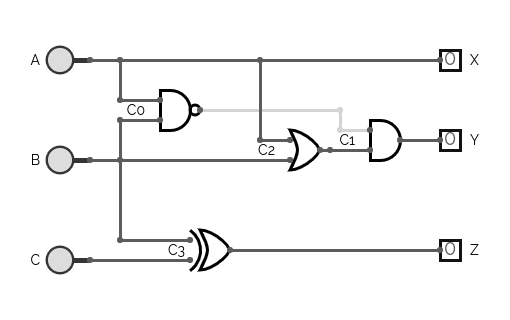
\includegraphics[width=0.5\textwidth]{circuit2}
	\end{figure}
	\begin{center}
		\begin{tabular}{ |C|C|C|C|C|C|C|C|C|C| } 
			\hline
			A & B & C & C_0 & C_1 & C_2 & C_3 & X & Y & Z \\
			\hline
			0 & 0 & 0 & 1 & 0 & 0 & 0 & 0 & 0 & 0 \\
			0 & 0 & 1 & 1 & 0 & 0 & 1 & 0 & 0 & 1 \\
			0 & 1 & 0 & 1 & 1 & 1 & 1 & 0 & 1 & 1 \\
			0 & 1 & 1 & 1 & 1 & 1 & 0 & 0 & 1 & 0 \\
			1 & 0 & 0 & 1 & 1 & 1 & 0 & 1 & 1 & 0 \\
			1 & 0 & 1 & 1 & 1 & 1 & 1 & 1 & 1 & 1 \\
			1 & 1 & 0 & 0 & 0 & 1 & 1 & 1 & 0 & 1 \\
			1 & 1 & 1 & 0 & 0 & 1 & 0 & 1 & 0 & 0 \\
			\hline
		\end{tabular}
		\hspace{0.5cm}
		\begin{tabular}{ l } 
			\hspace{0.5cm} It is obvious that: \\
			$X = A$ \\
			\hspace{0.5cm} Let us calculate: \\
			$Y = \bnot{A} \, B \, \bnot{C} + \bnot{A} \, B \, C + A \, \bnot{B} \, \bnot{C} + A \, \bnot{B} \, C =$ \\
			\hspace{0.25cm} $ = \bnot{A} \, B \, (\bnot{C} + C) + A \, \bnot{B} \, (\bnot{C} + C) =$ \\
			\hspace{0.25cm} $ = \bnot{A} \, B + A \, \bnot{B} = A \oplus B$ \\
			$Z = \bnot{A} \, \bnot{B} \, C + \bnot{A} \, B \, \bnot{C} + A \, \bnot{B} \, C + A \, B \, \bnot{C} =$ \\
			\hspace{0.25cm} $ = (\bnot{A} + A) \, \bnot{B} \, C + (\bnot{A} + A) \, B \, \bnot{C} =$ \\
			\hspace{0.25cm} $ = \bnot{B} \, C + B \, \bnot{C} = B \oplus C$ \\
		\end{tabular}
	\end{center}

\vspace{0.3cm}
To verify functional equivalence of two combinational circuits it is enough to prove that their inputs and outputs are \textbf{mappable} onto each other.
Mapping can be done using truth tables, for example. \\
The easiest way to do this will be putting inputs and outputs of the two circuit candidates in the same table:
\begin{center}
	\begin{tabular}{ |C|C|C|C|C|C|C|C|C| } 
		\hline
		A & B & C & X_1 & X_2 & Y_1 & Y_2 & Z_1 & Z_2 \\
		\hline
		0 & 0 & 0 & 0 & 0 & 0 & 0 & 0 & 0 \\
		0 & 0 & 1 & 0 & 0 & 0 & 0 & 1 & 1 \\
		0 & 1 & 0 & 0 & 0 & 1 & 1 & 1 & 1 \\
		0 & 1 & 1 & 0 & 0 & 1 & 1 & 0 & 0 \\
		1 & 0 & 0 & 1 & 1 & 1 & 1 & 0 & 0 \\
		1 & 0 & 1 & 1 & 1 & 1 & 1 & 1 & 1 \\
		1 & 1 & 0 & 1 & 1 & 0 & 0 & 1 & 1 \\
		1 & 1 & 1 & 1 & 1 & 0 & 0 & 0 & 0 \\
		\hline
	\end{tabular}
\end{center}
\end{proof}
